\documentclass[12pt]{article}
% REVISION NOTES %%%%%%%%%%%%%%%%%%%%%%%%%%%%%%%%%%%%%%%%%%%%
% 2008-0814 Location, Date, Time
% 2008-0814 fixed citations -- added bibliography.
%
%
\usepackage{geometry}                
\geometry{letterpaper}                   
%\geometry{landscape}                
\usepackage[parfill]{parskip}    
\usepackage{daves,fancyhdr,natbib,graphicx,dcolumn,amsmath,lastpage,url}
\usepackage{amsmath,amssymb,epstopdf,longtable}
\usepackage[final]{pdfpages}
\usepackage{paralist} 
\DeclareGraphicsRule{.tif}{png}{.png}{`convert #1 `dirname #1`/`basename #1 .tif`.png}
\pagestyle{fancy}
\lhead{CE 5333}
\rhead{FALL 2017}
\lfoot{CE 5333 -- Cleveland}
\cfoot{Page \thepage\ of \pageref{LastPage}}
\rfoot{DRAFT NO. 1}
\renewcommand\headrulewidth{0pt}
%%%%%%%%%%%%%%%%%%%%%%%%%%%%%%%%%%%%%%%%%%%%%%%%%%%%%%%
\begin{document}
\begin{center}
{\textbf{{ CE 5333 -- Special Topics in Water Resources}  {Exercise Set 5}}}
\end{center}
\begingroup
\begin{tabular}{p{1in} p{5in}}
Purpose: & Linear Programming  \\
\end{tabular}
\endgroup
%%%%%%%%%%%%%%%%%%%%%%%
\section*{\small{Exercise}}
\begin{enumerate}
\item A city is currently treating 8 MGD of wastes in a treatment plant and discharging 12 MGD of untreated waste into a river. 
A new plant is proposed.  
Figure \ref{fig:TreatmentPlants} is a schematic diagram of the overall treatment system.

\begin{figure}[htbp] %  figure placement: here, top, bottom, or page
   \centering
   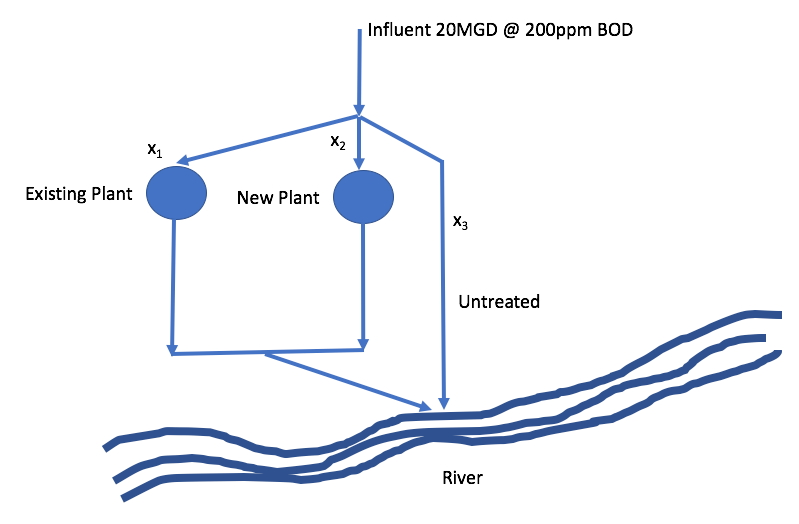
\includegraphics[width=6in]{TreatmentPlants.jpg} 
   \caption{Schematic of Treatment Plant Options}
   \label{fig:TreatmentPlants}
\end{figure}
The decision variables are:\\~\\
$x_1$ is the wastewater treated in the existing plant, in MGD.\\
$x_2$ is the wastewater treated in the new plant, in MGD. \\
$x_3$ is the wastewater discharged directly into the river (untreated), in MGD.\\

The existing plant has 80\% removal efficiency.  
The proposed plant will have 90\% efficiency.  
The existing plant has a maximum capacity of 8 MGD.

The Pollution Authority has recommended that the new 15 MGD plant be constructed. 
The plant will have a 30-year design life and a 5\% annual construction loan can be secured.
The Authority requires water to enter the river at a concentration of 25ppm BOD or less.
The city refuses to build the \$43.2 million facility because they claim the plant is too expensive.
Because the city has resisted, the Pollution Authority has imposed a fine of \$10,000 per day.
\begin{enumerate}[a)]
\item Determine the annual fine assuming the city pollutes the river 365 days/year.
\item Calculate annual payment on the 30 year loan to build the plant.
\item Compare the annual fine and construction costs.  Is it cheaper for the city to continue to pollute the river or to construct the plant.
\item Determine the water quality of the blended water (treated+untreated) from the existing plant.  Assume that $x_2=0$.
\end{enumerate}

\item The Pollution Authority wants to determine the effect of the fine upon the town's decision to treat its waste.
\begin{enumerate}[a)]
\item Determine the unit cost of the \$10,000 fine for untreated wastes (i.e.  \$10,000 = $c_3 \cdot x_3$, what is the value of $c_3$?) assuming the untreated waste discharge rate is 12 MGD at 200ppm BOD.
\item Build an LP model to minimize the total annual construction and fine costs for the town.  Consider the capacity of the current plant and the effluent flow of 20 MGD.  The capital unit cost to build the new plant as a function of the treatment flow rate through the new plant is 
$c_2= \$2.88 \times10^{6} \cdot x_2 $
\item Solve the LP model using \textbf{R} (or Excel).
\item Is the fine sufficient to make the building of the plant economically attractive?
\item What effect does doubling the fine have on the construction decision?
\end{enumerate}
\item If the Pollution Authority is required to change the water quality restrictions to a blended quality of 20ppm BOD or less, what is the best size and cost of the new facility, assuming the city does not wish to incur any non-compliance fine. 
\end{enumerate}


\end{document}


